\documentclass[tikz,border=5pt]{standalone}
\usepackage[utf8]{inputenc}
\usepackage[T1]{fontenc}
\usepackage{tikz}

\begin{document}

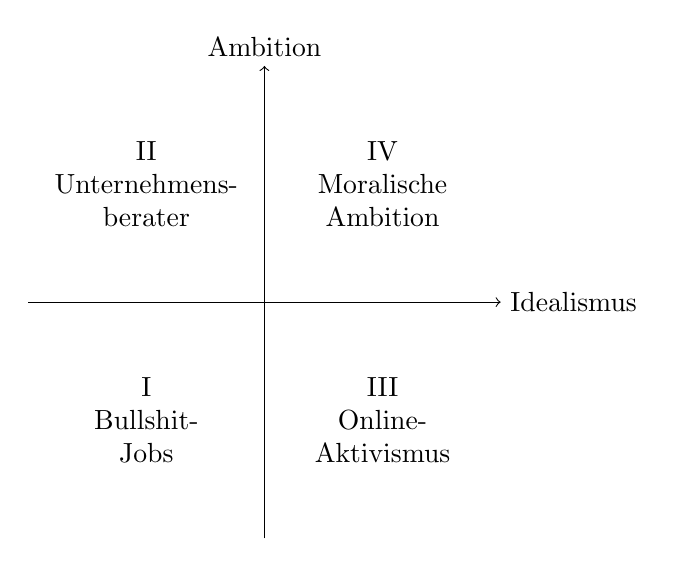
\begin{tikzpicture}[scale=1.5]
  \draw[->] (-2,0) -- (2,0) node[anchor=west] {Idealismus};
  \draw[->] (0,-2) -- (0,2) node[anchor=south] {Ambition};

  \tikzset{quadrant/.style={align=center}}

  \node[quadrant] at (1,1) {IV \\ Moralische \\ Ambition};
  \node[quadrant] at (1,-1) {III \\ Online- \\ Aktivismus};
  \node[quadrant] at (-1,-1) {I \\ Bullshit- \\ Jobs};
  \node[quadrant] at (-1,1) {II \\ Unternehmens- \\ berater};
\end{tikzpicture}

\end{document}
